\documentclass[12pt]{beamer}
\usepackage[T2A]{fontenc}
\usepackage[utf8]{inputenc}
\usepackage[english]{babel}
\usepackage{amssymb,amsfonts,amsmath,mathtext}
\usepackage{cite,enumerate,float,indentfirst}
\usepackage{longtable,xspace,subcaption}  
\usepackage{amsmath}
\usepackage{color}

\newcommand{\splitline}{\vspace{0.4cm}}
\graphicspath{{images/}}

\usetheme{Singapore}
\usecolortheme{beaver}

\setbeamercolor{footline}{fg=red}
\setbeamertemplate{footline}{
  \leavevmode%
  \hbox{%
  \begin{beamercolorbox}[wd=.333333\paperwidth,ht=2.25ex,dp=1ex,center]{}%
    Innopolis University
  \end{beamercolorbox}%
  \begin{beamercolorbox}[wd=.333333\paperwidth,ht=2.25ex,dp=1ex,center]{}%
    CloSpan
  \end{beamercolorbox}%
  \begin{beamercolorbox}[wd=.333333\paperwidth,ht=2.25ex,dp=1ex,right]{}%
  page \insertframenumber{} of \inserttotalframenumber \hspace*{2ex}
  \end{beamercolorbox}}%
  \vskip0pt%
}
\fontsize{9}{10}\selectfont
\newcommand\fontvi{\fontsize{10}{12}\selectfont}
\newcommand{\itemi}{\item[\checkmark]}
\title{\fontsize{15}{15}\selectfont
	\textbf{Mining Closed Sequential Patterns in Large Datasets
}}
\author{
	\fontvi
	\small{%	
\emph{Presenter:}~Ildar Nurgaliev\\%
\emph{Lab:}~Dainfos}\\%
}
\titlegraphic{
\includegraphics[width=0.2\linewidth]{iu}}
\date{}

\begin{document}

\maketitle

\begin{frame}{Main idea}
  Instead of mining the complete set of frequent subsequences we mine frequent \textit{closed subsequences}
\end{frame}

\begin{frame}{Definition of CS}{Frequent sequential pattern (FS) and closed FS (CS)}
\begin{itemize}
\item FS: includes all s of $\textit{support(s)} \ge \textit{min\_sup}$
\item $CS = \{ \alpha|\alpha \in~FS~and~\nexists\beta \in$ FS\\such that $\alpha \sqsubseteq \beta~and~support(\alpha) = support(\beta)\}$
\end{itemize}
\end{frame}

\begin{frame}{Definition of CS}{Example}
\begin{figure}
\center{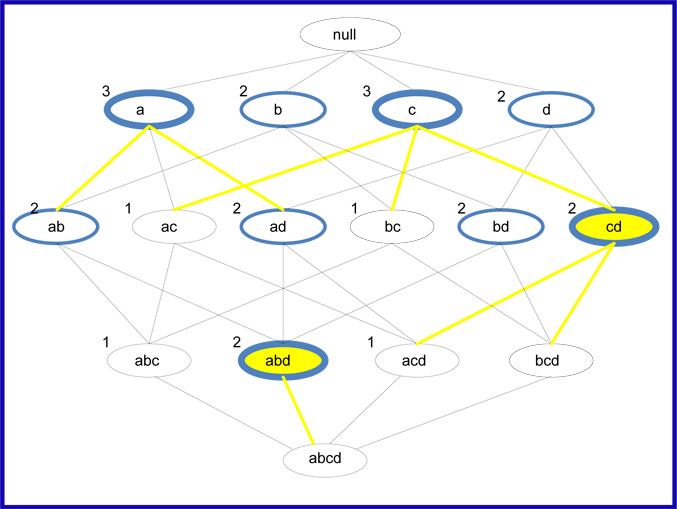
\includegraphics[width=0.6\linewidth]{cs_example}}
\end{figure}
\begin{itemize}
  \item circled \textcolor{blue}{blue} - Frequent
  \item the thick \textcolor{blue}{blue} - Closed Frequent
  \item filled yellow - Maximum Closed Frequent
\end{itemize}
\end{frame}

\begin{frame}{Mining CS}{Benefits}
\begin{itemize}
\item can mine really long sequences
\item produce significantly less number of discovered frequent sequences
\end{itemize}
\end{frame}

\begin{frame}{Dynamical Frequent Sequence Mining}{Why}
\begin{itemize}
  \item Traditional methods for data mining typically make the assumption that data is centralized and static.
  \item Such methods waste computational and I/O resources when data is dynamic and leads to cimmunication ovehead in distributed cas.
  \item As a result, the knowledge discovery process is harmed by slow response times.
  \item Efficient implementation of incremental data mining ideas in distributed computing environments is thus becoming crucial for ensuring scalability and facilitate knowledge discovery when data is dynamic and distributed.
\end{itemize}
\end{frame}

\end{document}